\chapter{The Adaptability Analyzer Software}
\label{cap:design}

To provide the software engineer a tool that can ease his work a new software has been developed ad hoc, called Adaptability Analyzer Tool\footnote{Source available at \url{https://github.com/TopoDiFogna/AdaptAnalyzer}}.

This tool has been developed from scratch with some goals in mind and puts together the previous SOLAR\cite{solar} metrics with the new metrics presented in Chapter \ref{cap:quality-metrics}. All the goals are explained in the following section.

A new feature was also implemented: the possibility to generate random architectures.

\section{Adaptability Analyzer Software Goals}
\subsection{User Point of View}
From a usability point of view the first goal of this software was to be a tool that can be used by every software engineer without knowing the underlying programming language or how the code is structured; to achieve this I've chosen to provide the software with a Graphical User Interface (GUI) that doesn't require any programming skill to be used.

Another goal was that creating an architecture and then perform calculations should be made easy for everyone, not only for the software engineer, so every result is clearly visible in the GUI and, where possible, numeric results are supported by Cartesian graphs and/or visual representations.

\subsection{Developer Point of View}
From a programming point of view, instead, the software has to be portable so it can be run on most computers, without strict limitations on operating systems and/or hardware. This is achieved by using the Java programming language\cite{java-se}. 

With this programming language the choices on how to develop the GUI were only two framework (discarding the old AWT\cite{awt}): Swing\cite{swing} or JavaFX\cite{javafx}. I've chosen to use the newer JavaFX because it should become the new standard for developing Java graphical applications and it provides a set of useful API to the scope of this software.

Others programming goals were to provide a software that can have a small memory footprint and low CPU usage but that can provide results in a meaningful time frame; this is achieved by using common design patterns with efficient algorithms in term of time and memory complexity.

The last goal was to make the user be able to export and import his architecture, thus interrupting and resuming his work on another machine is made easy.

More details on programming choices can be found in the Appendix \ref{app:usermanual}

\section{Adaptability Analyzer Software Features}

When launched, the tool presents a welcome page with the main menu accessible in the top left corner. From this menu it is possible to create a new architecture, either from scratch or generating one from the provided generator, or to import a previously created one as shown in Figure \ref{fig:welcome-screen-menu}

\begin{figure}[!ht]
	\centerline
	{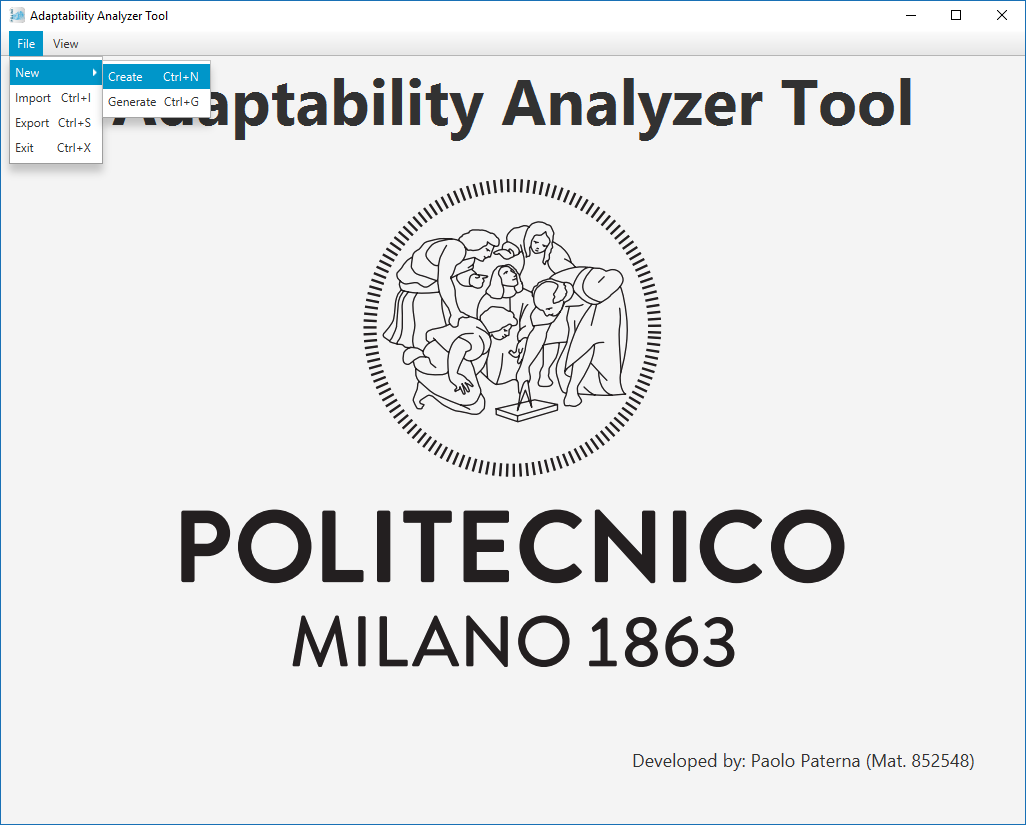
\includegraphics[scale=0.50]{img/welcome_screen_menu.png}}
	\caption[Tool Welcome Screen with Menu]{The main window of the tool that welcomes the user at launch with menu open.}
	\label{fig:welcome-screen-menu}
\end{figure}

When creating a new architecture from scratch the architecture's name is required as shown in Figure \ref{fig:new-arch} and then the main tool window, with the components tab open, is shown as in Figure \ref{fig:comp-details}. 

\begin{figure}[!ht]
	\centerline
	{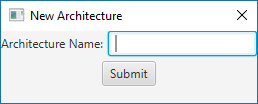
\includegraphics[scale=0.80]{img/new_arch.png}}
	\caption[New Architecture Window]{The new architecture window requesting only a name.}
	\label{fig:new-arch}
\end{figure}

\begin{figure}[!ht]
	\centerline
	{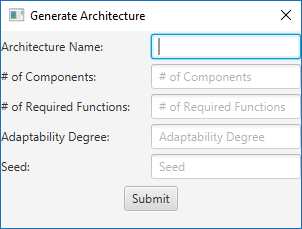
\includegraphics[scale=0.6]{img/gen_arch.png}}
	\caption[Generate Architecture Window]{The window that allow to generate an architecture.}
	\label{fig:gen-arch}
\end{figure}

\begin{figure}[!ht]
	\centerline
	{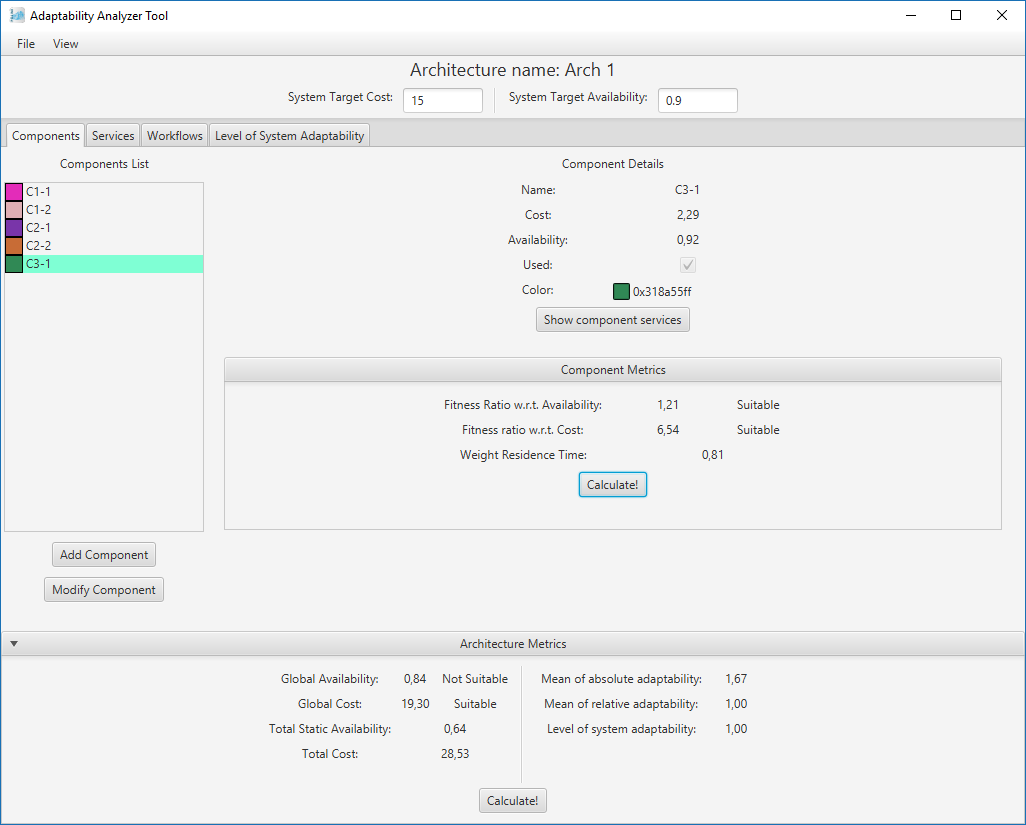
\includegraphics[scale=0.50]{img/comp_details.png}}
	\caption[Component Details Window]{The main tool window showing all the component details.}
	\label{fig:comp-details}
\end{figure}

When generating an architecture instead some more parameters are required and are summarized in Table \ref{tab:gen-parameters}, the window is shown in Figure \ref{fig:gen-arch}

\begin{table}[ht!b]
	\centering
	\begin{tabular}{|l|l|}
		\hline
		\multicolumn{1}{|c|}{Parameter name} & \multicolumn{1}{c|}{Meaning} \\
		\hline 
		Architecture name & Name of the architecture \\
		\hline
		\# of Components & The number of components that the architecture should have \\
		\hline
		\# of Required Functions & The number of functions every component should require \\
		\hline
		Adaptability Degree & How many copies of the same component should be \\
		\hline
		Seed & Random number to regenerate the same architecture multiple times \\
		\hline
		
	\end{tabular} 
	\caption[Generator Parameters]{The parameters required by the architecture generator.}
	\label{tab:gen-parameters}
\end{table}

In this case the architecture is named \emph{Arch 1} and the component \emph{C3-1} is selected from the list of available components on the right, visible because it is highlighted. Every component in the list can be deleted by right clicking on it and selecting delete from the context menu. On the left it is possible to see all the component details. All the fields are explained in Table \ref{tab:comp-details}.

\begin{table}[ht!b]
	\centering
	\begin{tabular}{|l|l|}
		\hline
		\multicolumn{1}{|c|}{Parameter name} & \multicolumn{1}{c|}{Meaning} \\
		\hline 
		Component name & Name of the selected component \\
		\hline
		Cost & Cost of the component \\
		\hline
		Availability & Availability of the component as specified in its technical features\\
		\hline
		Used & If the component is active in the architecture \\
		\hline
		Color & The color used in the graphical representation \\
		\hline
		
	\end{tabular} 
	\caption[Component Parameters]{The parameters required by the component creator.}
	\label{tab:comp-details}
\end{table}

If the top fields, \emph{System Target Cost} and \emph{System Target Availability} are filled as described in Chapter \ref{cap:quality-metrics} Section \ref{sec:new-metrics} and at least one component exists, it is already possible to calculate all the component metrics, shown on the right just below the component details, and architecture metrics shown on the bottom of the tool pressing the respective buttons. The meaning of this metrics are explained in Chapter \ref{cap:quality-metrics}.

It is also possible to add a new component or modify an existing one by pressing the respective button under the components list; in this case the window that is opened is the same but in case of modifying a component the fields are already filled as shown in Figure \ref{fig:add-modif-comp}

\begin{figure}[!ht]
	\centerline
	{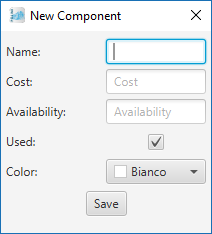
\includegraphics[scale=0.6]{img/add_modif_comp.png}}
	\caption[Add/Modify Component]{The window that is shown when adding or modifying a component.}
	\label{fig:add-modif-comp}
\end{figure}

Now is possible to navigate all the other features of the tool.
 
From the top menu, in the \emph{View} section, it is possible to view a graphical representation of the architecture as shown in Figure \ref{fig:view-arch} and from there it is possible to export an image of such representation. 

The nodes can be rearranged inside the window by dragging and dropping them.

\begin{figure}[!ht]
	\centerline
	{\includegraphics[scale=0.50]{img/view_arch.png}}
	\caption[Architecture Graphical Representation]{The graphical representation of the architecture in example.}
	\label{fig:view-arch}
\end{figure}

The service tab shown in Figure \ref{fig:serv-details} allows to choose a component from the drop-down menu on the left and a service it provides or requires. It is also possible here to add a service to the selected component by pressing the corresponding button on the bottom of the list as shown in Figure \ref{fig:add-serv}. Every service can be deleted by right clicking on it and selecting delete from the context menu.

Once selected a service its details are displayed on the right; if some detail does not apply for the selected service it is grayed out automatically. The meaning of the details are explained in Table \ref{tab:serv-details}

\begin{table}[ht!b]
	\centering
	\begin{tabular}{|p{3,5cm}|p{9cm}|}
		\hline
		\multicolumn{1}{|c|}{Parameter name} & \multicolumn{1}{c|}{Meaning} \\
		\hline 
		Name & Name of the selected service \\
		\hline
		Type & If the service is \emph{Required} or \emph{Provided} by the component \\
		\hline
		Execution Time & Time to execute if this service is called (only provided services)\\
		\hline
		Used Probability & The probability that this service is needed by a call (only required services)\\
		\hline
		Number of Executions per Call & The number of executions the service must do before giving a result (only required services) \\
		\hline
		
	\end{tabular} 
	\caption[Service Parameters]{The parameters required by the service creator.}
	\label{tab:serv-details}
\end{table}


\begin{figure}[!ht]
	\centerline
	{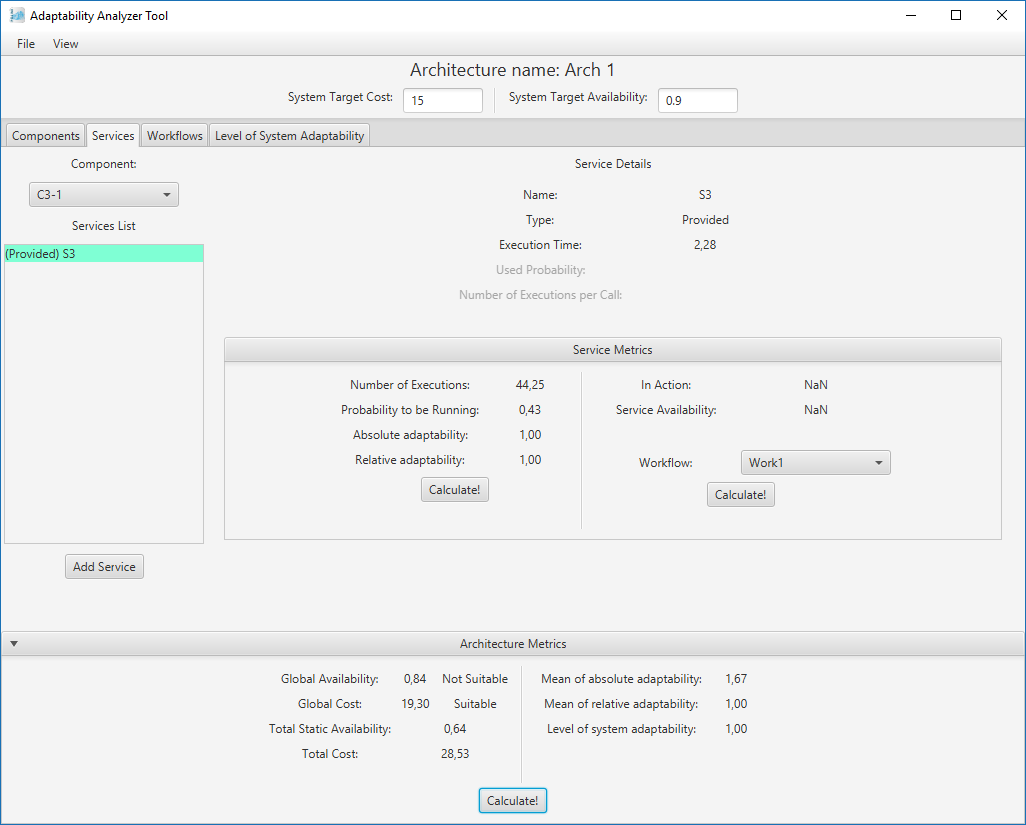
\includegraphics[scale=0.50]{img/serv_details.png}}
	\caption[Service Details Tab]{The main tool window showing all the service details.}
	\label{fig:serv-details}
\end{figure}

\begin{figure}[!ht]
	\centerline
	{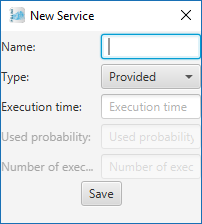
\includegraphics[scale=0.6]{img/add_serv.png}}
	\caption[Add Service Window]{The window that is shown when adding a service.}
	\label{fig:add-serv}
\end{figure}

The Workflow tab allows to create different workflows for the architecture; it is shown in Figure \ref{fig:workflow-path1}. Every workflow is represented as a Sequence Diagram from the UML Standard \cite{uml}. Each workflow has one or more paths that can be created using the corresponding button below the path list. Every workflow or path can be deleted by right clicking on it and selecting delete from the context menu. 

If an \texttt{Alt} and/or \texttt{Opt} block are needed that can be specified by additional paths which on creation require an execution probability. The only limitation is that \texttt{Alt} and \texttt{Opt} blocks can't be nested in the actual implementation.

The execution probability is shown on top of the left side of the tab and below that is possible to add a message with the corresponding button. The window that allows to create a message is shown in figure \ref{fig:message}

To delete a message and all its successor just click on the arrow.

\begin{figure}[!ht]
	\centerline
	{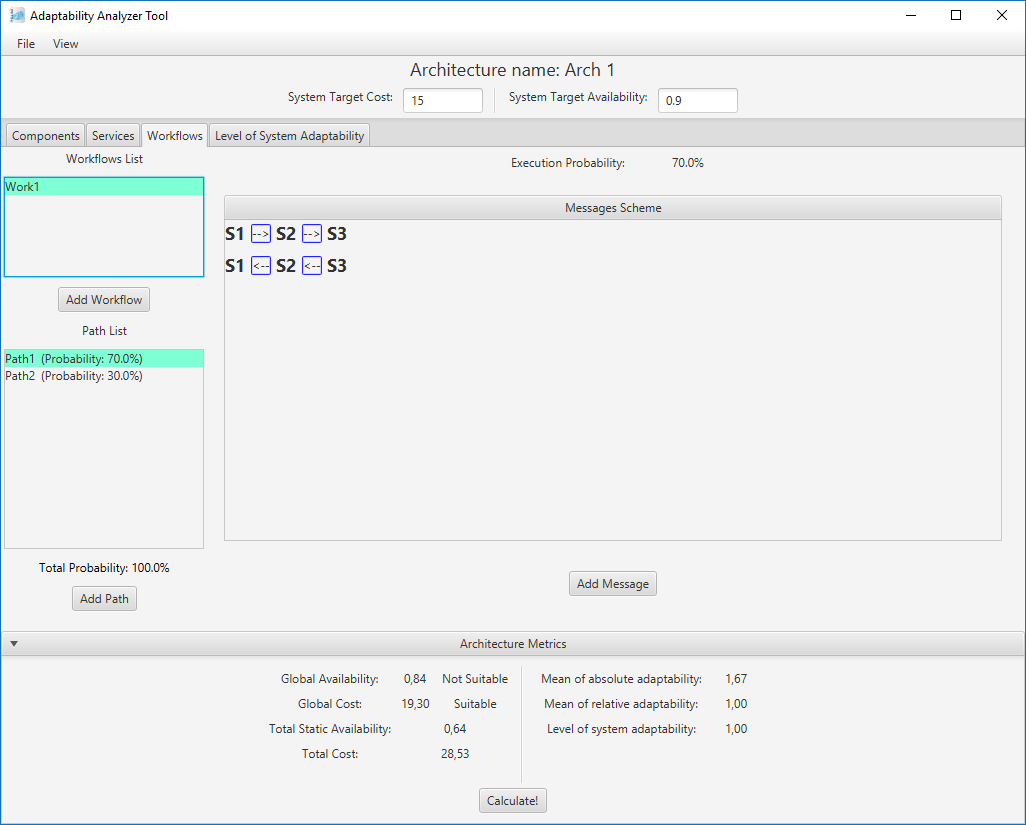
\includegraphics[scale=0.50]{img/work1path1.png}}
	\caption[Workflows Tab]{The main tool window showing workflows, paths and the sequence diagram.}
	\label{fig:workflow-path1}
\end{figure}

\begin{figure}[!ht]
	\centerline
	{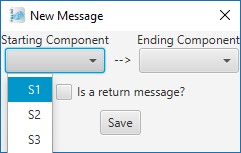
\includegraphics[scale=0.6]{img/message.png}}
	\caption[Add Path Window]{The window that is shown when adding path.}
	\label{fig:message}
\end{figure}

The last tab is the Level of System Adaptability Tab. In this tab it is possible to calculate all possible architectures that can exists with the given components and calculate how the cost varies with respect to the adaptability as shown in Figure \ref{fig:adapt-wrt-avail}. 

\begin{figure}[!ht]
	\centerline
	{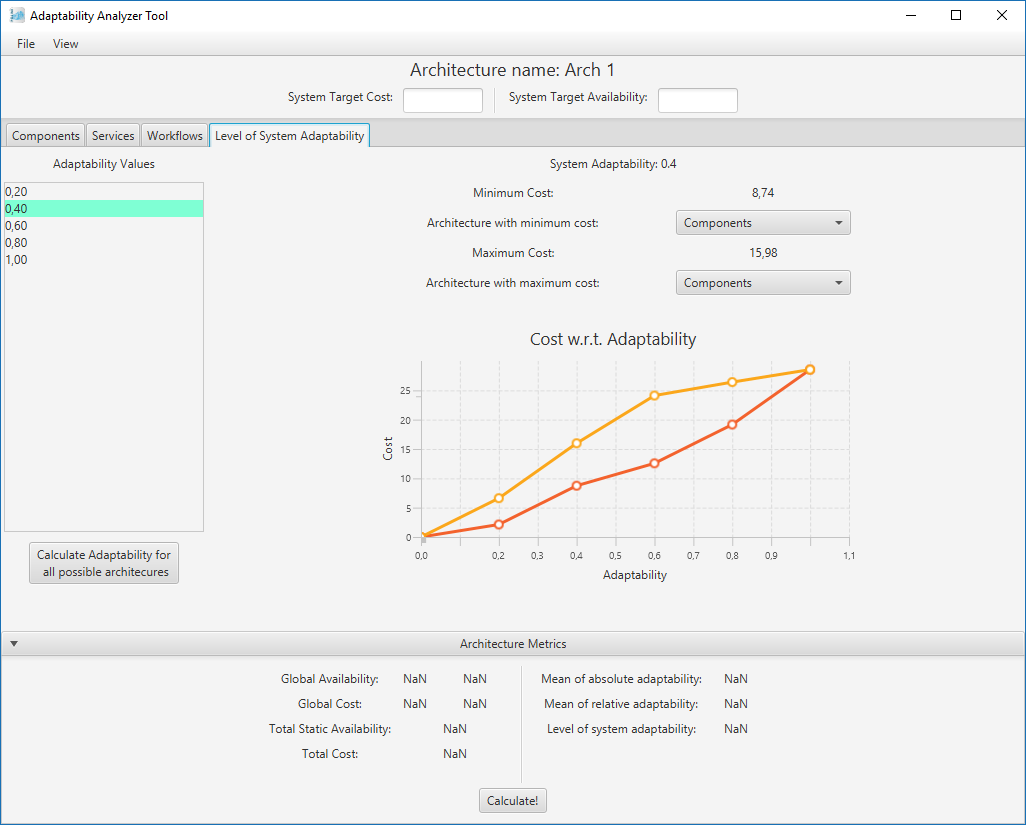
\includegraphics[scale=0.50]{img/adapt_wrt_avail.png}}
	\caption[Availability Window]{The window that is shown when adaptability calculated.}
	\label{fig:adapt-wrt-avail}
\end{figure}

Clicking an adaptability value in the list on the left or a dot in the graph selects a possible adaptability value and displays on the right the minimum and maximum cost for that adaptability and the list of components that are in the architecture with the selected adaptability as shown in Figure \ref{fig:adapt-wrt-avail-comp}. 

Selecting a component the component tab is shown with te selected component visible.

\begin{figure}[!ht]
	\centerline
	{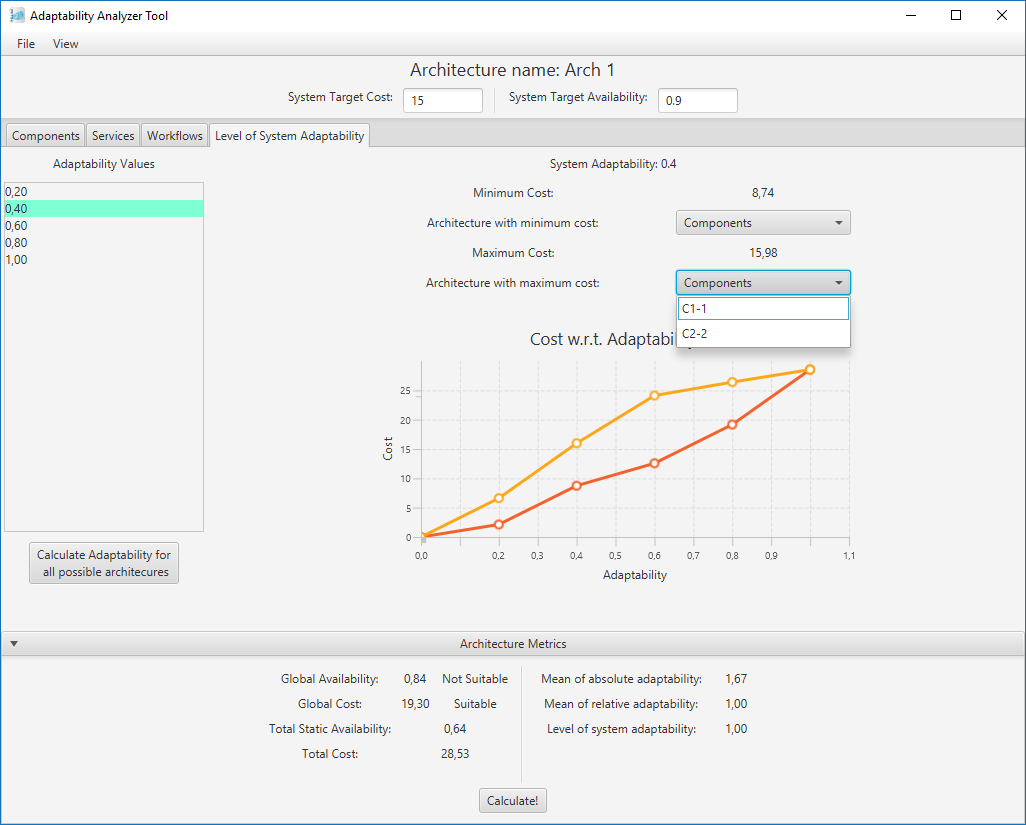
\includegraphics[scale=0.50]{img/adapt_wrt_avail_comp.png}}
	\caption[Availability Window with Architecture]{An architecture shown for a selected adaptability.}
	\label{fig:adapt-wrt-avail-comp}
\end{figure}
